\chapter{関連研究}
\label{related_works}
\section{概要}
コンピュータ工学研究者のFelsは、オブジェクトと人との関係性を、「Embodiment」の観点から4つに分類した\cite{Fels}。
「Embodiment」については、認知科学やコンピュータ科学の理論用語にも同じ名前のものが存在する。中でも参照されることの多いものとして、認知科学者・哲学者である Gallagher\cite{Gallagher2000} の「ミニマルセルフ」という考え方が挙げられる。\\
Gallagherの「ミニマルセルフ」についての論文が発表されたのは2000年で、同時にFelsがこの分類を行ったのも同じ2000年であり、FelsがGallagherの考えを参照していたのかはわからないが、Felsの捉えるEmbodimentは、「ミニマルセルフ」の説明とも重なる部分があり、相反する理論ではないと考える。さらにFelsのEmbodimentは、人とオブジェクトとの関係について「一体化 (Embodiment) していない状態」についても言及している。これは、\ref{introduction}章に提起した「技量の問題」による「使いづらさ」について説明する上で有効な分類である。\\
そこで本章ではまず、Gallagherの「ミニマルセルフ」とFelsによるEmbodimentを説明し、両者の関係について整理する。その上で、Felsの分類から改めて「技量の問題」による「使いづらさ」を説明し、それに着目した本研究が、Embodimentに着目している先行研究や作品と比べた上での、相違点について述べる。

\section{Gallagherのミニマルセルフ}
認知科学者・哲学者のGallagher\cite{Gallagher2000}は、自己を構成する2つの要素として、ミニマルセルフ(最小限の自己)とナラティヴ・セルフ(物語的自己)があると説明した。中でも「ミニマルセルフ」とは、一切の自己知識を失ったとしても残る最小限の自己であり、身体所有感(sense of ownership, body ownership)、行為主体感(sense of agency)の二つによって支えられていると説明する。\\
こうしたGallagherの分類に基づき、それらを評価する方法が考案され、ラバーハンド錯覚実験などにみられるように、生来の肉体ではないものを自分の身体と錯覚してしまうような、人間の身体像の曖昧さに注目した研究が認知科学や心理学の領域で取り組まれてきた。\\
こうした研究で蓄積された実証的知見は、インターフェースデザインや身体拡張の設計・評価へと応用されている。インターフェース研究者の渡邊は、機械や情報処理が介在する高度で複雑な道具であっても、「使っている最中にはその道具自体を意識せずに身体の一部になったかのようになり、目的に集中できる」こと、すなわち「道具の透明化」という、ヒューマンインターフェースの理想を実現するための指針としてこの概念に注目する。渡邊は、例えばマウスカーソルやスマートフォンのような「操作時の指とグラフィックの追従性が高い」インターフェースには「自己帰属感(Gallagherのsense of ownershipに対する訳語)」が生じるとし、このことからこうしたインターフェースは「自身の一部、延長」として考えられ、「道具の透明化」が実現すると説明する\cite{Watanabe2013}\cite{Watanabe2017}。

\section{FelsのEmbodiment}
Felsは、オブジェクトと人との関係性について、Reponse、Control、Gontemplation、Belongingの4つに分類した。それぞれの説明は以下の通りである。

\textbf{Response:}\\
オブジェクトに対する働きかけの結果から、感情的な反応や理解を得る状態を指す。Felsはこの関係性の例として「コンピュータとそれに初めて触れた人」を挙げ、「なんらかの操作を通して得られた、便利な機能に喜んでいる状態。また逆に、有用な結果を得られず落胆する状態」と説明する。

\textbf{Control:}\\
人がオブジェクトを自分自身の延長として使用し、その操作によって感情的な満足や美的体験を得る状態を指す。Felsは、自身の作品であるIamascopeにおいて、人の身体動作にシステムが素早く視覚的なフィードバックを返すことから、こうした関係性が生じると説明する。「自分自身の延長」として経験される感覚について言及しており、またそれが追従性の高いグラフィックによってもたらされるという記述は、渡邊がマウスカーソルやスマートフォンに対して用いた「操作時の指とグラフィックの追従性が高い」インターフェースという説明と同等のものである。このことからFelsのいうControlとは、Gallagherの「sense of ownership」と同じものを指していると考えられる。

\textbf{Contemplation:}\\
人がオブジェクトに対する働きかけはせず、人がそのオブジェクトからの信号やメッセージを内省や反映を通じて体験する状態を指す。Felsはその具体例として、絵画の鑑賞体験を挙げる。

\textbf{Belonging:}\\
オブジェクトによって人が動かされているような経験を指す。人はそのオブジェクトによって提供される体験を通じて感情的な反応を得る。ここでは、オブジェクトが人の体験や感情を形作る役割を果たす。

\section{FelsのIntimacy}
さらにFelsは、オブジェクトと人とのあいだにある「深い関係」を指して、「Intimacy」という尺度で説明する。例えば楽器と人の関係性ように、Intimacyのある関係性のもとでは、「あたかもその装置が身体の延長であるかのように、考えや感情を効果的に表現できる」という。上記の、FelsによるEmbodimentの分類においては、ResponseとControlが、それぞれIntimacyの低い状態、高い状態として説明ができる。

以降の節では、このIntimacyの観点から、近年取り組まれている身体性の変容に着目した研究や作品について整理し、本研究・制作の位置付けを示す。

\section{本研究の位置付け}
FelsのいうIntimacyは、初めてオブジェクトと人とが出会ったときから、関係性が変化することで到達できる状態である。Fels自身が語る通り、FelsのIamascopeという作品はIntimacyが生じるまでの期間が短い一方で、楽器や自転車といったオブジェクトと人とのあいだにIntimacyが生じるまでの期間は比較的長く、試行錯誤や使い手の興味が重要になってくる。一言にIntimacyと言ってもそれが生じるまでの期間には違いがあるが、本節ではこの「期間」の違いについて整理することで、本研究の位置付けを整理したい。

\begin{figure}[H]
  \centering
  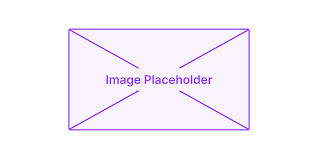
\includegraphics[width=15cm]{img/placeholder.png}
  \caption{本研究の位置付け}
  \label{fig:position}
\end{figure}

FelsのいうIntimacyの考えに基づいてこれらの事例を考えると、これらが扱うIntimacyの経験は、「錯覚」「コントローラブル」な経験として説明できる。ラバーハンド実験のような「錯覚」体験については、頭で理解していても抗えないほど強いIntimacyを引き出す体験となっている。一方で、楽器のような道具と人とのあいだには、習得のための練習を経てようやく、Intimacyが生じる。楽器習得に関して言えば、演奏したい曲や弾きこなしたいフレーズが想起できているのに、思うように扱うことができないことから、そのギャップに「もどかしさ」を経験することがある。このようなIntimacyは、必ずしも楽しさだけでなく、不快さを伴う経験でもある。その過程に「もどかしさ」を経験することが特徴的な、こうしたIntimacyを扱う研究は、まだ少ない。\\
そこで、本研究ではこうした過程を\textit{grasp}と名付けた。
\textit{grasp}は「把握」を意味する動詞・名詞だが、日本語でも物体を把持する手の動作であると同時に、概念について理解するときにも用いる。ここでの\textit{grasp}とは、「人がある対象に注意や目的意識を抱き、注意を向けた対象を確かめるため、または目的の達成に向けて試行を行う期間」のことを指す。手指の構造を変化させる本作は、このコンセプトに注目し、手指の変換をきっかけに起こる注意や、変換した手指とボールとの関係のもとで生じる目的意識が、体験者の中で自発的に生まれることを目指した。
本研究では、作品体験についてのインタビューを通してそれが実現していたことを示し、そのデザインプロセスと最終的な作品形態についての考察を通して、\textit{grasp}の設計に向けた指針となることを目指す。

\section{身体性の変容に着目した研究}
自在肢プロジェクト、えくす手、親指の動きを肩の動きにマッピングさせる実験など、VRやロボティクスの分野でも取り組まれている研究では「sense of agency」や「sense of ownership」に基づく評価・設計が行われている。



\section{身体性の変容を扱った作品}
モデルトラッキングを用いて身体性の変容を扱った作品はいくつか存在する。小川らによる「えくす手(Metamorphosis Hand)」\cite{ekusute}では、指の伸びた手などの現実の身体にはあり得ない特性を持ったバーチャルな身体を通じてピアノを演奏することができる。そのねらいは、「現実とは異なる特性のバーチャルハンドへの身体所有感の生起を通じ、現実の身体的制約を超えたインタラクションを実現する、一種のバーチャルな身体拡張体験を提供する」と説明される。\\
身体所有感の生起要因に関するこれまでの議論を参照し、本作は「テクスチャ、形状、空間的配置、解剖学的構造の4つの特性」を根拠に、身体所有感が生じながらも、自己身体と意味的に類似しないバーチャルハンドを制作している。これらの特性は、身体所有感を生じさせる上での実証的知見ではあるが、本研究が対象とするIntimacyは、例えば楽器のように、こうした生起要因を押さえなくとも、習得を経て生じうるのではないかと考える。また、生起要因を多く踏襲しているわけではないからこそ、身体所有感が生じるまでには期間を必要とし、その程度にも個人差が生じるのではないだろうか。これらの観点から、本研究の取り組みは「えくす手」よりも極端な身体変容を促す体験として位置付けられる。\\
佐藤雅彦らによる「君の身体を変換してみよ展」はさまざまなアプローチで身体の変容を扱う作品が展示されたが、その中でも「点にんげん・線にんげん」という作品は、ボディトラッキングを用いて取得された全身の関節の位置を捉えたキーポイントが点として扱われ、異なる方法で結びつけられたり、ボロノイ分割が適用される点群として扱われるなど、さまざまな「変換」が行われている。\\
本作品との構造上の相違点として、関節の位置を捉えたキーポイントの並び替えの有無が挙げられる。佐藤らの作品では、身体の関節の位置を捉えたキーポイントはその配置を変えることなく、繋げ方やインターフェースの文脈における位置付けの違いで展開される。一方、本作ではキーポイントの配列もダイナミックに変化する。これは、手指が複雑な動きのできる器官であると同時に、身体の中でもっとも随意に動かすことのできる器官でもあることから、構造が大きく異なる場合でも、手指の動きに連動している箇所を、動かしている中で容易に同定できると考えているためである。


